\documentclass[a4paper]{article}
\usepackage[pdftex]{graphicx,color}
\usepackage[hidelinks]{hyperref}
\usepackage{anysize}
\usepackage[utf8]{inputenc}
\usepackage[T1]{fontenc}
\usepackage[portuguese,brazil]{babel}
\usepackage{fancyhdr}
\usepackage{natbib}
\usepackage{amssymb}
\usepackage{amsmath}
\usepackage{subfig} % Figuras lado a lado.
\usepackage{mathptmx} % Usa fonte tipo times new roman
\usepackage{tabularx} % tabelas mais flexíveis
\usepackage{titlesec} % possibilita alterar o formato das seções
\usepackage{parskip} % controle de espaçamento de parágrafos
\usepackage{colortbl} % Changes colors in tables
\usepackage{caption} %Possibilita editar captions.
\usepackage{float}
\usepackage{fontawesome}

\captionsetup{%
    ,format=hang
    ,justification=raggedright
    ,singlelinecheck=false
    ,figureposition=top
    }

%%%%%%%%%%%%%% Formatação dos estilos das seções
\titleformat{\section}
 {\normalfont\Large\bfseries}{\thesection.}{0.5em}{}[{\titlerule[0.6pt]}]

%%%%%%%%%%%%% Tabela
\captionsetup[table]{name=Quadro} %Altera o nome de Tabela para Quadro.


%%%%%%%%%%%%% Apelidos para bibliografias
\newcommand{\mnras}{Mon. Not. R. Astron. Soc.}
\newcommand{\aap}{Astronomy $\&$ Astrophysics}
\newcommand{\apjs}{ApJS}
\newcommand{\apj}{Astrophys. J.}
\newcommand{\apjl}{Astrophys. J. Letters}
\newcommand{\aj}{Astron. J.}
\newcommand{\pasa}{PASA}
\newcommand{\nat}{Nature}
\newcommand{\natastron}{Nature Astronomy}

%%%%%%%%%%%%%%%% Espaçamento entre linhas
\renewcommand{\baselinestretch}{1.5} % Espaçamento de 1.5 entre linhas
\setlength{\parskip}{10pt} % espaço entre parágrafos (uma linha em branco).

%%%%%%%%%%%%%% Margens
%\marginsize{left}{right}{top}{bottom}
\marginsize{30mm}{20mm}{30mm}{20mm}

%%%%%%%%%%%%% Cabeçalho e rodapé
\pagestyle{fancy}
\fancyhf{} % clear all fields
\fancyhead[R]{
	Universidade Federal do Espírito Santo\\ 
	Programa Institucional de Iniciação Científica \\
	Relatório Final de Pesquisa\\
	\textcolor{black}{Ciências Exatas e da Terra (CNPq)}
}
\rfoot{\thepage}
\renewcommand{\headrulewidth}{0pt}

%%%%%%%%%%%%%%%%%%%%%%%%%%%%
%%%%%%%%%%%% Begin Document
\begin{document}

\vspace*{.01cm}

\begin{center}
 {\Large \bf  \textcolor{black}{Análise de matéria escura em grandes levantamentos de galáxias - Piic/Ufes}}
 \end{center}

\vspace{.5cm}

\begin{tabularx}{\textwidth}{|>{\columncolor[gray]{0.9}} l|X|}
\hline
{\bf Edital:} & \textbf{Edital Piic 2024 / 2025} \\
\hline
{\bf Área do Conhecimento (CNPq):} & Ciências Exatas e da Terra  \\
\hline
{\bf Subárea do Conhecimento (CNPq):} & Física \\
\hline
{\bf Título do Projeto:}& Gravitação além de relatividade geral: teoria e análise de dados astrofísicos  \\
\hline
{\bf Título do Subprojeto:} & Análise de matéria escura em grandes levantamentos de galáxias\\
\hline
{\bf Professor Orientador:} & Davi Cabral Rodrigues\\
\hline
{\bf Estudante:} & Matheus Agenor Gomes da Costa\\
\hline
\end{tabularx}

\vspace{.5cm}

%%%%%%%%%%%%%%%%%%%%%%%%%%%%%
\section{Introdução}
Galáxias são objetos compostos essencialmente por 3 componentes bariônicas\footnote{Define-se bariônica toda a matéria composta por bárions, como prótons e nêutrons, formando a matéria "comum".}, Estrelas, Gás e Poeira, e uma componente não bariônica conhecida como matéria escura (por exemplo Hernandez-Arboleda \& Rodrigues, 2021). Historicamente, a componente de Matéria Escura foi primeiro proposta por Zwicky (1933, 1937) e revisitada por Bosma (1978) e Rubin (1978) de forma independente. Diversas observações atualmente apontam para a existência da matéria escura, que aparece nas escalas de galáxias, aglomerados de galáxias e do universo observável como um todo. Embora haja ampla evidência sobre sua existência a partir de diferentes meios de detecção, por exemplo, dinâmica interna de galáxias e lentes gravitacionais, para todos os efeitos a matéria escura é sempre detectada através da interação gravitacional (Binney \& Tremaine, 2011; Keeton, 2014).

O modelo cosmológico atual $\Lambda$CDM ($\Lambda$ \textit{cold dark matter}) tem grande sucesso em prever uma série de questões observacionais em grande escala, mas também apresenta problemas sistemáticos em escalas galácticas, dentre eles podemos citar o problema \textit{cuspe-núcleo} (\textit{cusp-core}) (De Blok, 2010; Del Popolo \textit{et al}, 2014). As simulações baseadas em $\Lambda$CDM sugerem um perfil de densidade de matéria escura quase universal, um perfil que decai com $r^{-3}$ em grandes raios (Navarro, Frenk \& White, 1997). Tal perfil de densidade, conhecido como Navarro-Frenk-White (NFW), é dado por:
\begin{equation}
\rho_{\text{NFW}}(r) = \frac{\rho_s}{\frac{r}{r_s} \left(1 + \frac{r}{r_s}\right)^2},
\end{equation}
onde $\rho_s$ é a densidade característica e $r_s$ é o raio de escala. Este modelo é caracterizado por uma densidade que aumenta de forma acentuada em direção ao centro do halo (uma "cúspide"). Entretanto, para galáxias anãs e de baixo brilho superficial, esse perfil parece não satisfazer as observações, que frequentemente indicam um "núcleo" de densidade constante. Um perfil fenomenológico importante que descreve tal comportamento é o perfil de Burkert (1995), dado por:
\begin{equation}
\rho_{\text{Burkert}}(r) = \frac{\rho_0}{\left(1 + \frac{r}{r_c}\right)\left(1 + \frac{r^2}{r_c^2}\right)},
\end{equation}
onde $\rho_0$ é a densidade central e $r_c$ é o raio de núcleo. Para raios pequenos ($r\ll r_c$), a densidade se aproxima de um valor constante, formando o núcleo.

Para investigar a estrutura dos halos de matéria escura, este trabalho utilizou dados do catálogo SPARC (\textit{Spitzer Photometry and Accurate Rotation Curves}; Lelli, McGaugh \& Schombert, 2016). O catálogo combina fotometria em $3.6\,\mu$m do Telescópio Espacial Spitzer com curvas de rotação de alta qualidade, derivadas de observações de hidrogênio atômico (H\,I) e, em alguns casos, de H$\alpha$, para 175 galáxias próximas. Os dados fornecem as contribuições de velocidade do gás, do disco estelar e do bojo, permitindo a construção de modelos de massa detalhados.

A metodologia empregada evoluiu de uma análise preliminar baseada em busca em grade (\textit{grid search}) e minimização de $\chi^2$ para uma abordagem mais sofisticada de inferência Bayesiana, utilizando técnicas de Monte Carlo via Cadeias de Markov (MCMC). Este método permitiu uma exploração robusta do espaço de parâmetros de quatro perfis de matéria escura (NFW, Burkert, Einasto e Pseudo-Isotérmico), com o objetivo de determinar qual modelo descreve melhor os dados observacionais.

%%%%%%%%%%%%%%%%%%%%%%%%%%%%%
\section{Materiais e Métodos}
A metodologia deste trabalho foi desenvolvida para permitir uma inferência robusta dos parâmetros que descrevem os halos de matéria escura, utilizando um arcabouço de análise Bayesiana. O processo completo abrange desde a seleção dos dados observacionais até a implementação de algoritmos numéricos para amostragem do espaço de parâmetros e critérios estatísticos para a comparação de modelos teóricos.

\subsection{Especificações dos Dados e da Amostra}
A análise empírica deste trabalho fundamenta-se inteiramente no banco de dados \texttt{SPARC} (\textit{Spitzer Photometry and Accurate Rotation Curves}). Este catálogo consiste em uma amostra de 175 galáxias próximas, abrangendo uma vasta gama de propriedades, incluindo morfologias (de S0 a Irregulares), luminosidades (aproximadamente 5 ordens de magnitude) e brilhos superficiais (aproximadamente 4 ordens de magnitude). Essa diversidade torna o \texttt{SPARC} uma amostra representativa de galáxias de disco no universo local, ideal para o estudo de relações de escala e dinâmica galáctica.

A componente cinemática do \texttt{SPARC} é composta por curvas de rotação de alta qualidade, compiladas a partir de mais de 30 anos de observações interferométricas de Hidrogênio neutro (H\,I). O H\,I é um traçador ideal do potencial gravitacional, pois é dinamicamente frio, segue órbitas aproximadamente circulares e se estende muito além do componente estelar, permitindo sondar regiões onde a matéria escura é dominante.

Para aproximadamente um terço da amostra (56 galáxias), as curvas de rotação são híbridas, combinando dados de H\,I nas regiões externas com dados de H$\alpha$ nas partes internas. Os dados de H$\alpha$, obtidos com espectroscopia de fenda longa, unidades de campo integral (IFUs) ou interferometria Fabry-Perot, possuem alta resolução espacial ($\sim$1''), o que minimiza os efeitos de \textit{beam-smearing} e permite uma medição mais precisa das velocidades de rotação internas.

A fotometria para todas as 175 galáxias foi obtida de forma homogênea a partir de imagens do Telescópio Espacial Spitzer no infravermelho próximo, especificamente na banda de [3.6] $\mu$m. Esta banda é um excelente indicador da massa estelar, pois a razão massa-luminozidade ($\Upsilon_{*}$) apresenta variações muito menores do que em comprimentos de onda ópticos e depende fracamente da história de formação estelar da galáxia. O processamento das imagens incluiu a limpeza interativa de fontes contaminantes (estrelas de primeiro plano e galáxias de fundo) e uma estimativa cuidadosa do céu de fundo, que representa a fonte dominante de incerteza fotométrica.

O catálogo \texttt{SPARC} fornece diretamente os modelos de massa para os componentes bariônicos, ou seja, as contribuições para a curva de rotação do gás ($V_{\text{gas}}$), do disco estelar ($V_{\text{disk}}$) e do bojo ($V_{\text{bul}}$). A contribuição do gás é calculada a partir dos perfis de densidade de H\,I, assumindo uma massa total de $1.33 \times M_{HI}$ para incluir a contribuição de Hélio. A contribuição estelar é calculada a partir do perfil de brilho superficial. Para galáxias com tipo de Hubble anterior a Sbc ($T<4$), foi realizada uma decomposição bojo-disco para separar a luz do bojo e do disco (mais detalhes sobre as caracteristicas das galaxias do catalogo podem ser encontradas em Lelli et al., 2016).

\subsection{Estrutura de Análise Bayesiana}
A inferência dos parâmetros foi conduzida dentro do formalismo Bayesiano, cujo pilar é o Teorema de Bayes:
\begin{equation}
    P(\theta|D) = \frac{P(D|\theta) P(\theta)}{P(D)},
\end{equation}
onde $P(\theta|D)$ é a distribuição posterior, $P(D|\theta)$ é a verossimilhança (\textit{likelihood}), e $P(\theta)$ é a priori (\textit{prior}). Assumindo que as incertezas nos dados são Gaussianas, a verossimilhança logarítmica ($\ln\mathcal{L}$) é proporcional à estatística qui-quadrado ($\chi^2$):
\begin{equation}
    \ln\mathcal{L} \propto -\frac{1}{2} \chi^2(\theta) = -\frac{1}{2} \sum_{i=1}^{N} \frac{\left(V_{\text{obs},i} - V_{\text{total},i}(\theta)\right)^2}{\sigma_i^2}.
\end{equation}
A velocidade total do modelo, $V_{\text{total}}$, é a soma em quadratura de todos os componentes (gás, disco, bojo e halo). Um prior Gaussiano em escala logarítmica foi aplicado à razão massa-luz do disco ($\Upsilon_{\text{D}}$), com centro em $0.5\,(M_\odot/L_\odot)_{[3.6 \mu m]}$ e um desvio padrão de 0.1 dex.

\subsection{Implementação Numérica e Comparação de Modelos}
Para mapear a distribuição posterior, foi implementado um processo de duas etapas. Primeiramente, utilizou-se o algoritmo de Evolução Diferencial para encontrar o mínimo global da função de custo (equivalente ao máximo da verossimilhança), garantindo uma inicialização robusta para a segunda etapa. Em seguida, a distribuição posterior foi amostrada com o método de Monte Carlo via Cadeias de Markov (MCMC), utilizando o amostrador de conjunto afim-invariante da biblioteca Python \texttt{emcee}. Este método é altamente eficiente para amostrar distribuições com fortes correlações entre parâmetros.

Para avaliar qual perfil de matéria escura melhor descreve os dados, foi utilizado o Critério de Informação Bayesiano (BIC), que penaliza modelos com maior número de parâmetros livres ($k$):
\begin{equation}
    \text{BIC} = k \ln(N) + \chi^2_{\text{min}},
\end{equation}
onde $N$ é o número de pontos de dados. O modelo com o menor valor de BIC é considerado o mais parcimonioso e, portanto, o preferível.

%%%%%%%%%%%%%%%%%%%%%%%%%%%%%
\section{Resultados e Discussão}
A metodologia de inferência Bayesiana foi aplicada a uma amostra de oito galáxias do catálogo \texttt{SPARC}, dividida entre quatro galáxias de alto brilho superficial (HSB) e quatro de baixo brilho superficial (LSB). Esta seção detalha os resultados da comparação entre os modelos de halo de matéria escura e discute suas implicações no contexto da estrutura galáctica.

\subsection{Comparação dos Perfis de Matéria Escura}
A análise comparativa entre os quatro perfis de matéria escura (NFW, Burkert, Einasto e Pseudo-Isotérmico) revelou uma clara preferência dos dados por modelos com um perfil de densidade interno suave ou com núcleo. Como sintetizado no Quadro \ref{tab:best_models}, o Critério de Informação Bayesiano (BIC) indicou que os perfis de Burkert e Einasto forneceram o melhor ajuste em todos os casos analisados. A amostra dividiu-se precisamente, com quatro galáxias (duas HSB e duas LSB) favorecendo o perfil de Burkert e as outras quatro (duas HSB e duas LSB) favorecendo o perfil de Einasto.

\begin{table}[H]
    \centering
    \caption{Melhor modelo de halo de matéria escura para cada galáxia da amostra, de acordo com o Critério de Informação Bayesiano (BIC). A análise também fornece os parâmetros de melhor ajuste para a massa do halo ($M_{200}$) e a razão massa-luz do disco ($\Upsilon_{\text{D}}$).}
    \label{tab:best_models}
    \begin{tabular}{l c c c c}
        \hline
        \textbf{Galáxia} & \textbf{Classe} & \textbf{Melhor Modelo} & \textbf{log$_{10}(M_{200})$} & \textbf{$\Upsilon_{\text{D}}$} \\
        & & & $[M_{\odot}]$ & $[M_{\odot}/L_{\odot}]$ \\
        \hline
        NGC3521 & HSB & Burkert & $11.90^{+0.07}_{-0.10}$ & $0.57$ \\
        NGC5005 & HSB & Burkert & $11.77^{+0.15}_{-0.19}$ & $0.49$ \\
        UGC03546 & HSB & Einasto & $11.21 \pm 0.05$ & $0.31$ \\
        UGC08699 & HSB & Einasto & $11.86^{+0.10}_{-0.21}$ & $0.51$ \\
        \hline
        NGC0055 & LSB & Einasto & $10.24^{+0.09}_{-0.06}$ & $0.51$ \\
        NGC2366 & LSB & Einasto & $9.34^{+0.05}_{-0.04}$ & $0.47$ \\
        NGC3109 & LSB & Burkert & $10.76^{+0.06}_{-0.06}$ & $0.53$ \\
        UGC05721 & LSB & Burkert & $10.32^{+0.04}_{-0.04}$ & $0.56$ \\
        \hline
    \end{tabular}
\end{table}

É particularmente notável que em nenhum dos casos o perfil NFW, canonicamente associado ao modelo $\Lambda$CDM, foi o preferido. Este resultado reforça diretamente a tensão conhecida como "problema cúspide-núcleo". A preferência pelo perfil de Burkert, que é definido por um núcleo de densidade constante, e pelo perfil de Einasto, cuja flexibilidade permite modelar um declive de densidade mais suave no centro, sugere que os halos de matéria escura de galáxias reais são estruturalmente diferentes das previsões de simulações que consideram apenas a matéria escura fria. Os ajustes das curvas de rotação para todos os modelos e para as amostras HSB e LSB são ilustrados na Figura \ref{fig:rotation_curves}.

\begin{figure}[!ht]
    \centering
    \begin{minipage}[b]{0.48\textwidth}
        \centering
        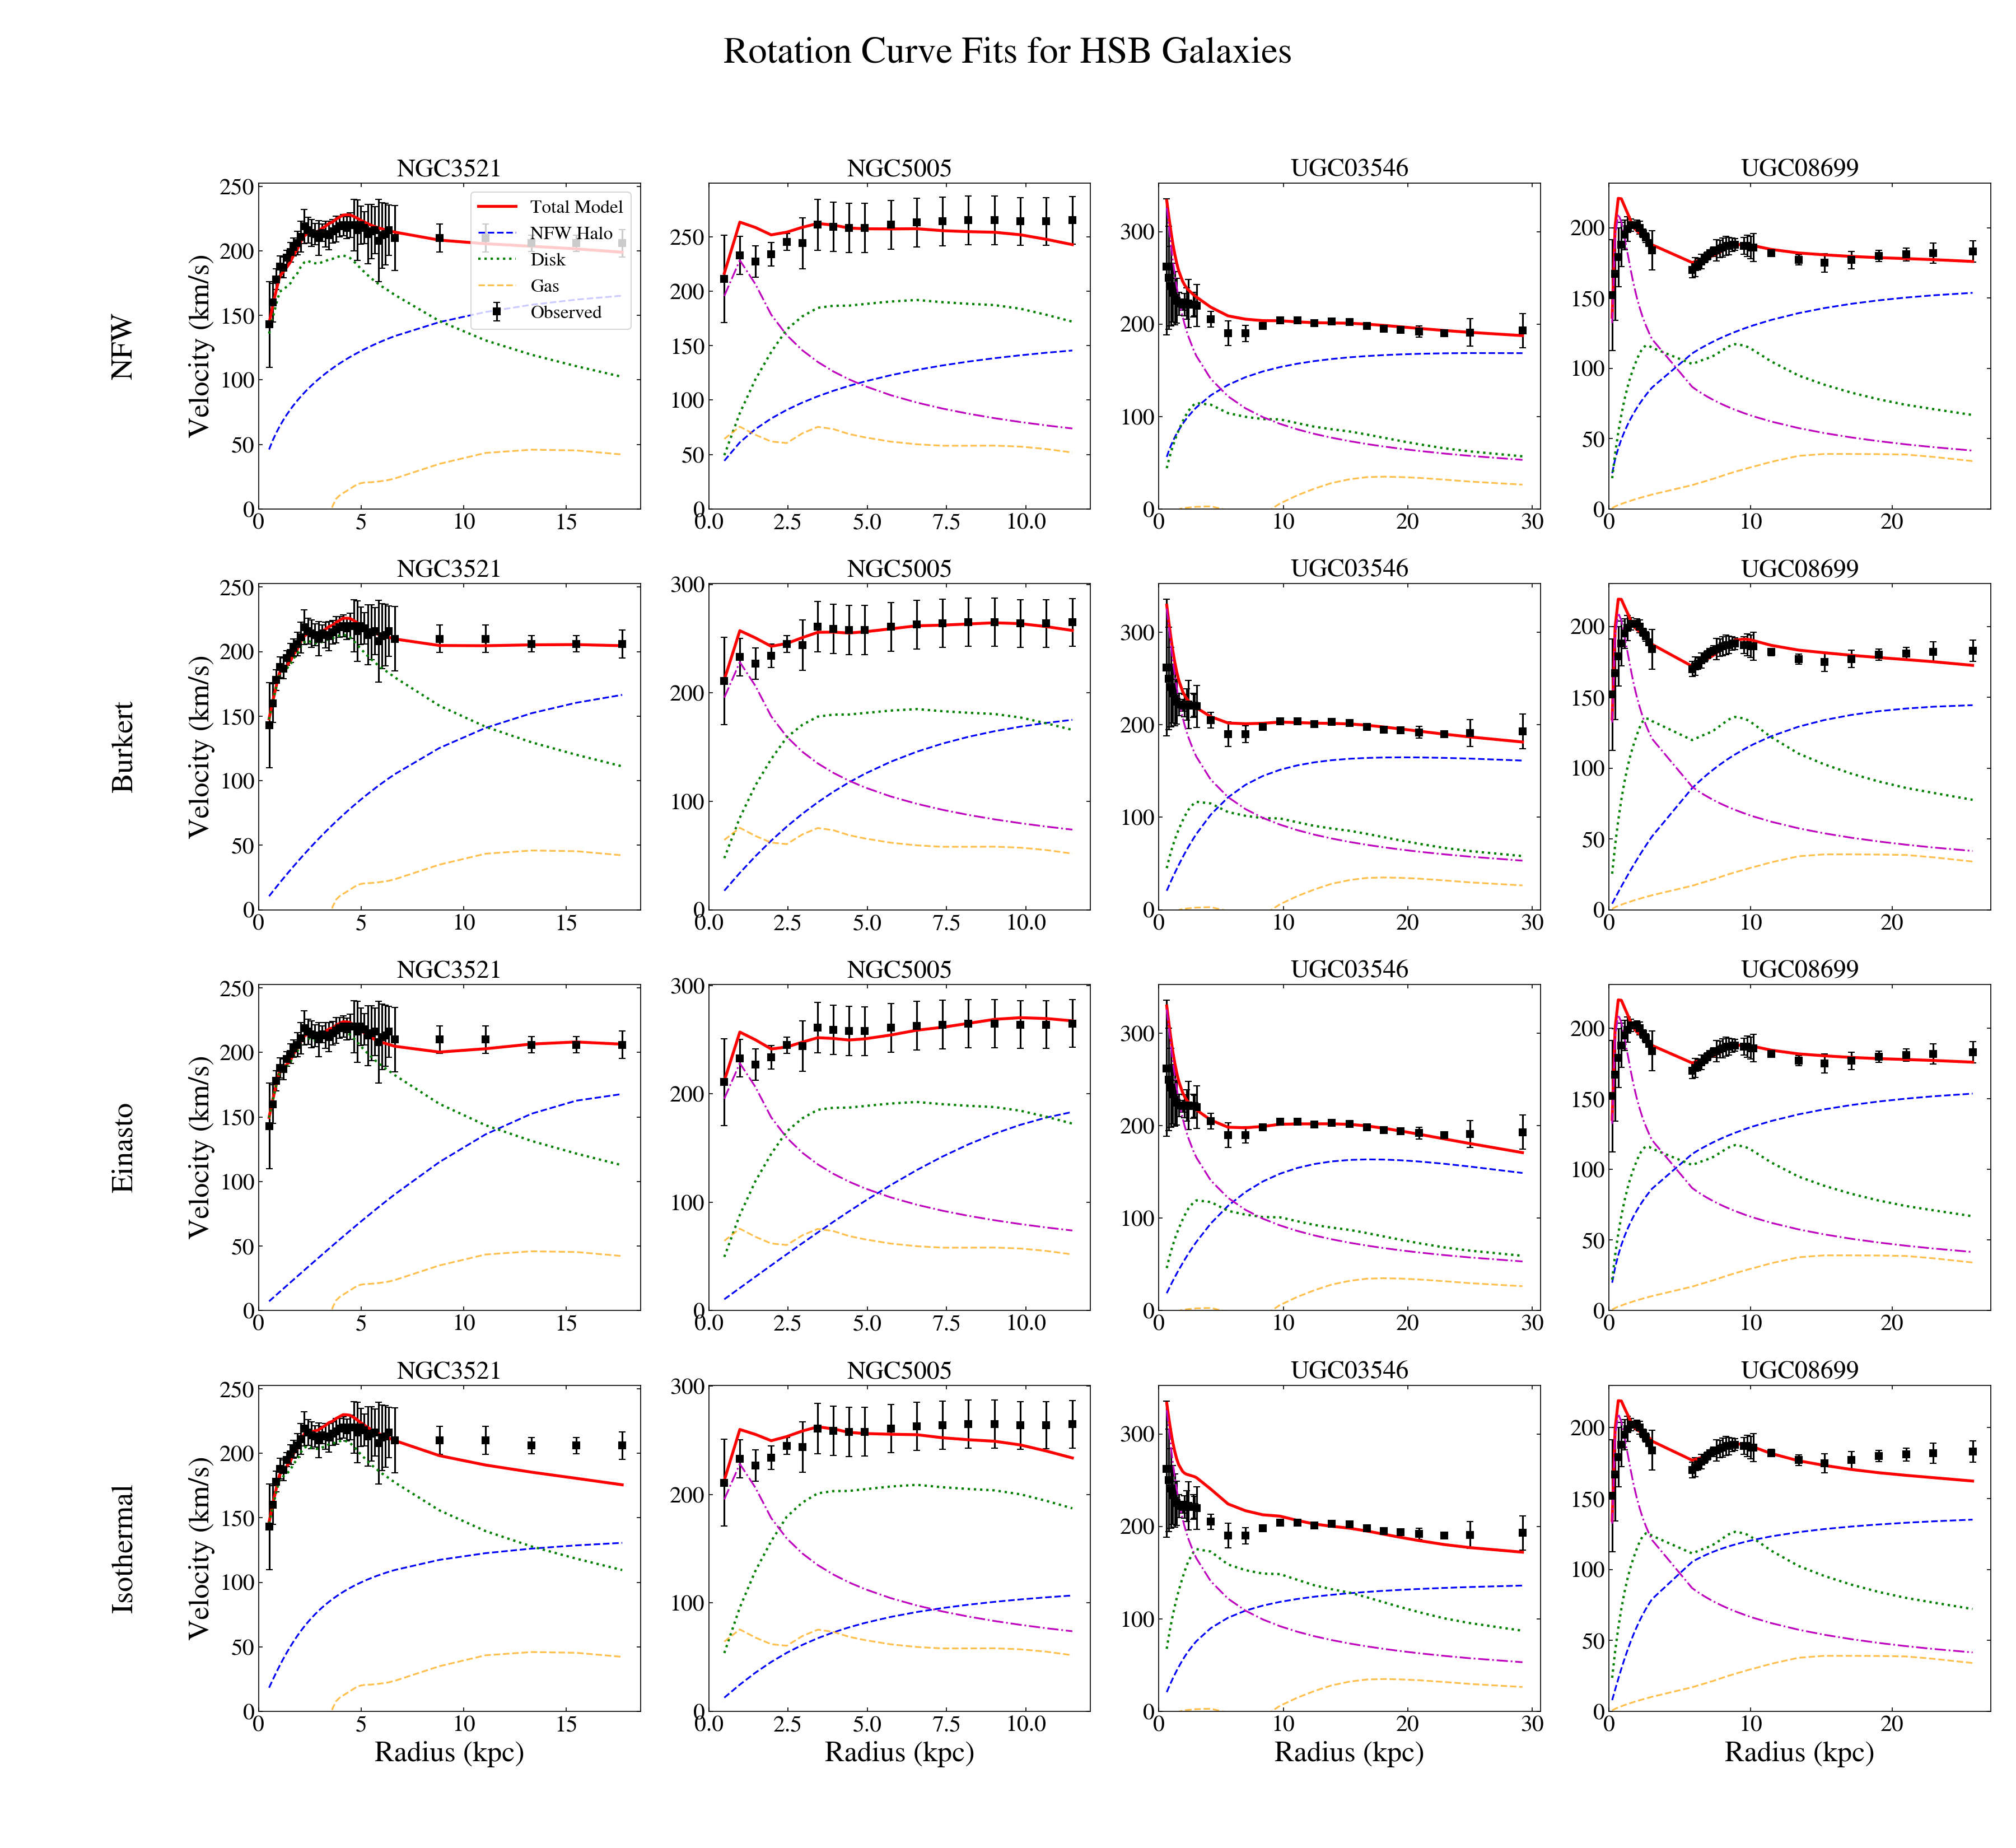
\includegraphics[width=\textwidth]{figs/diagnostic_rotation_curves_HSB.png}
    \end{minipage}
    \begin{minipage}[b]{0.48\textwidth}
        \centering
        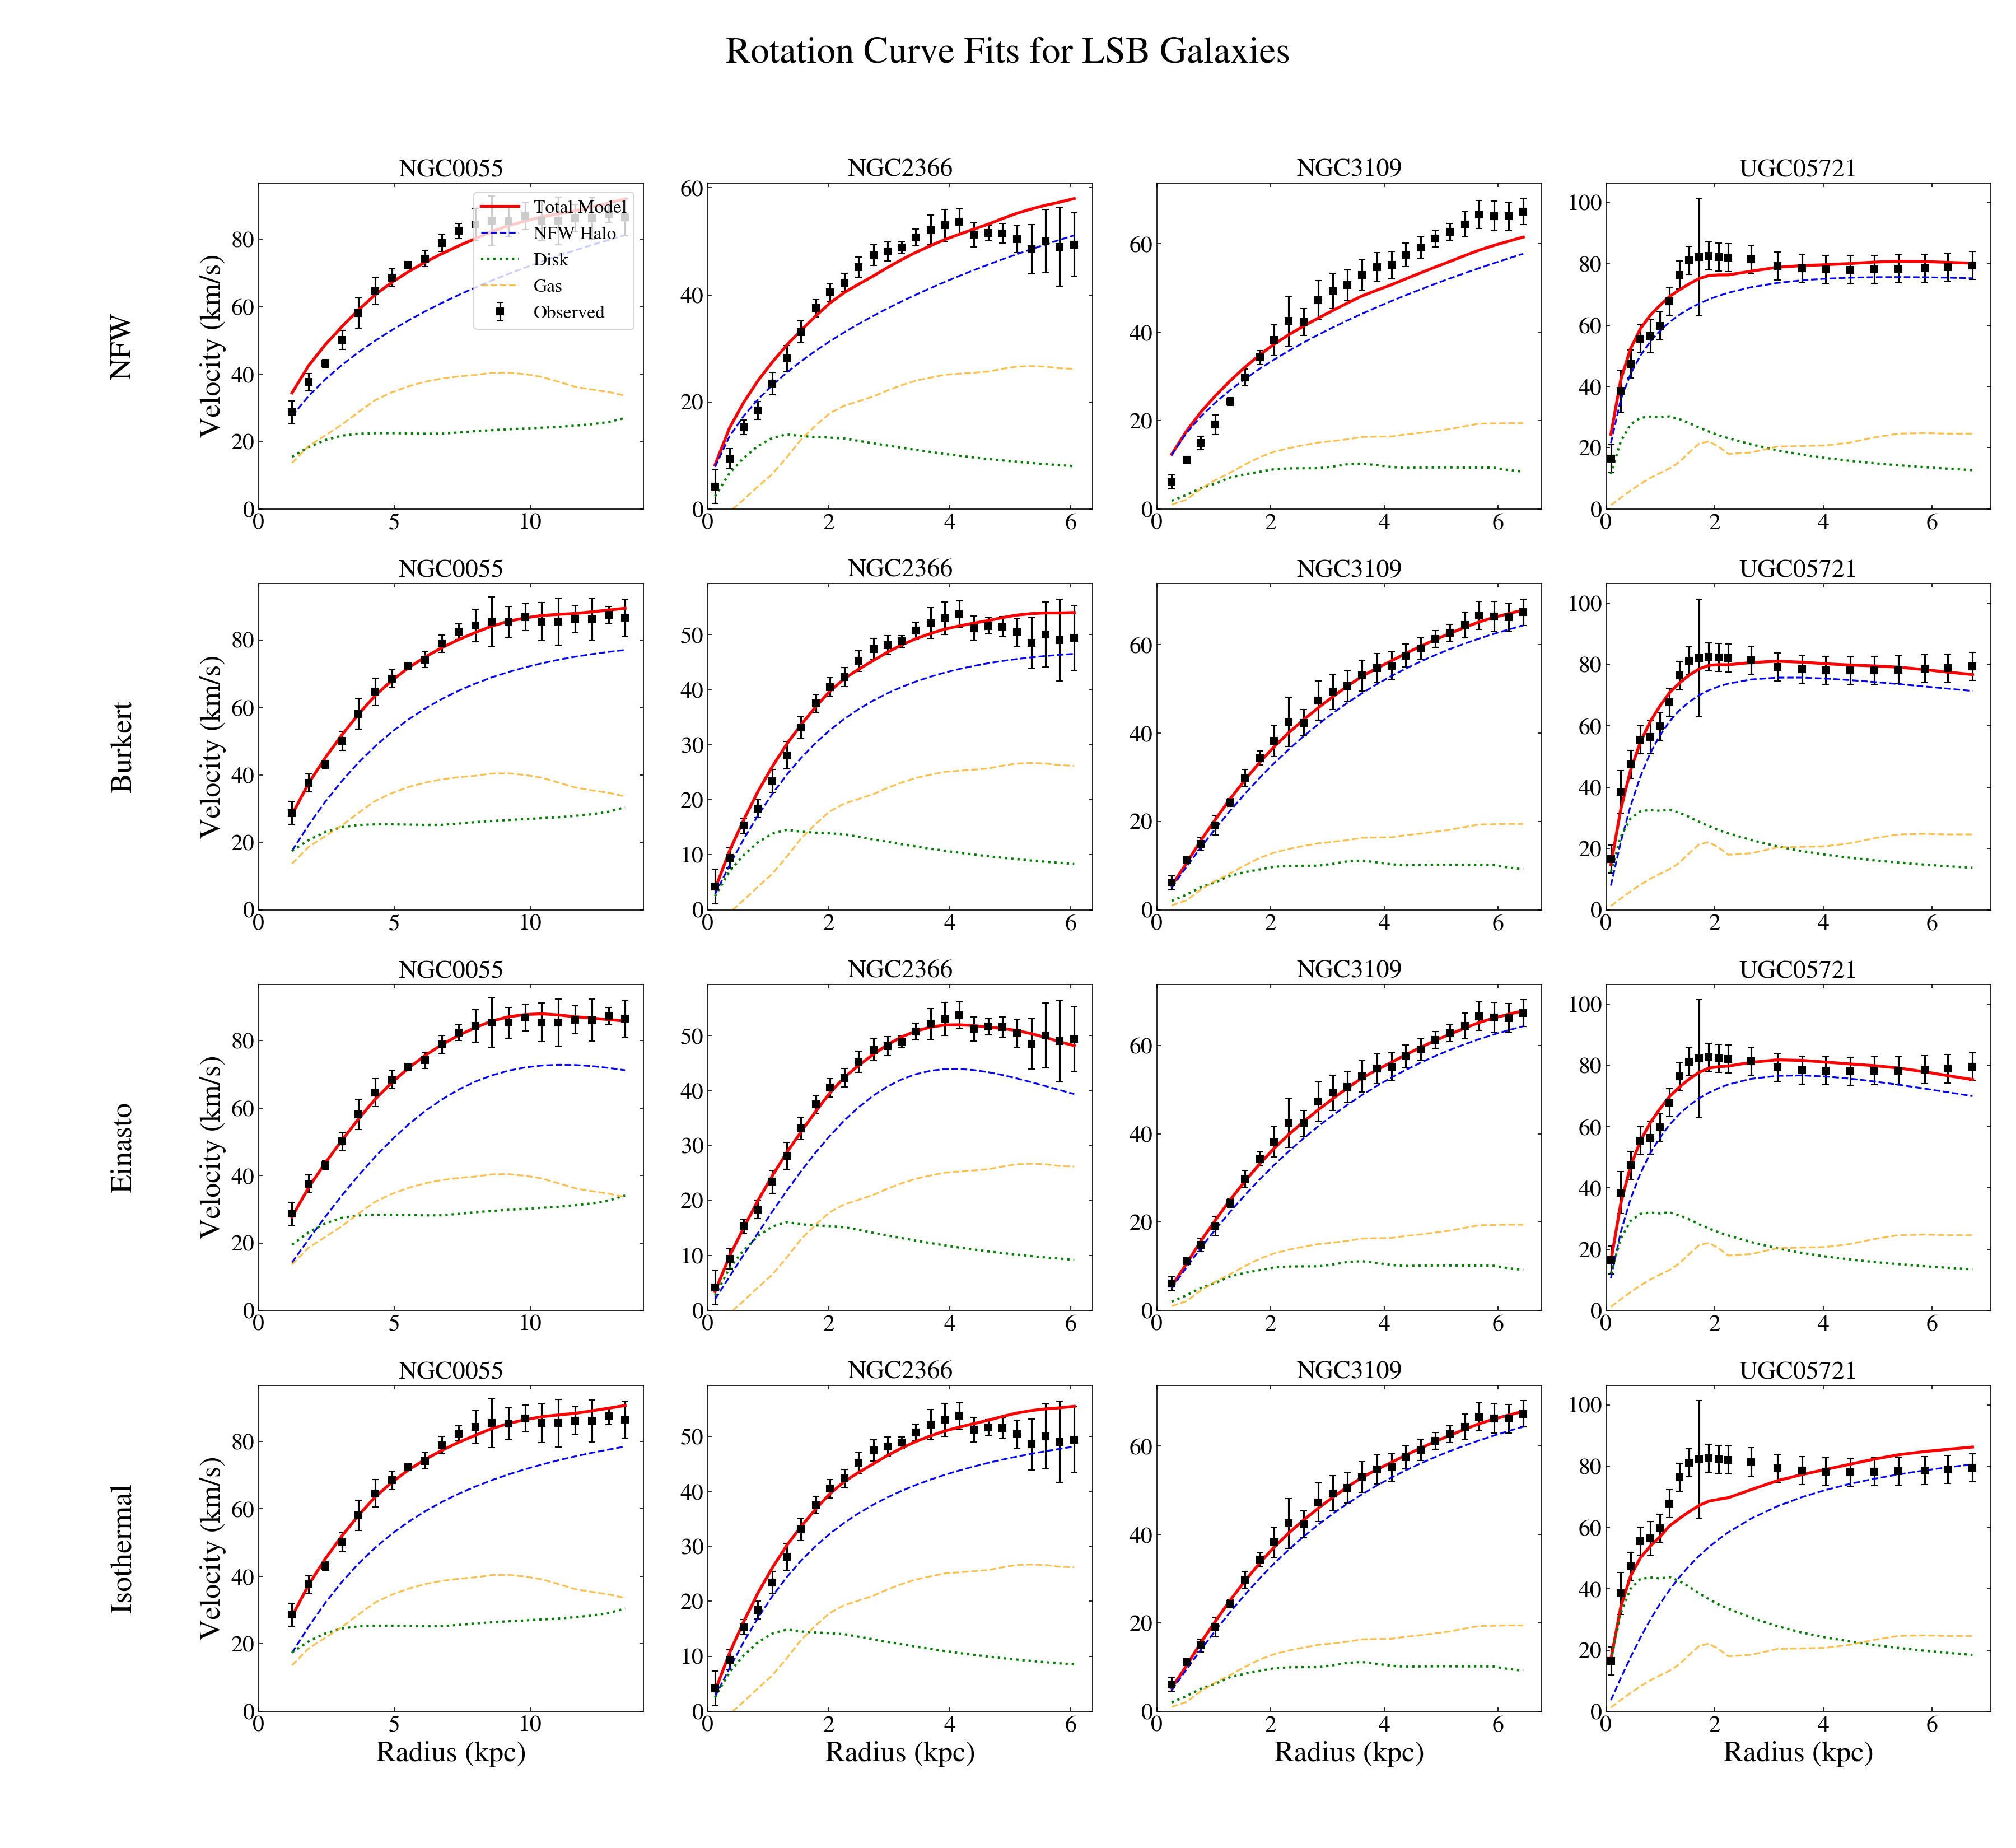
\includegraphics[width=\textwidth]{figs/diagnostic_rotation_curves_LSB.png} 
    \end{minipage}
    \caption{Ajustes das curvas de rotação para os quatro modelos de matéria escura em galáxias de alto (HSB, painel da esquerda) e baixo (LSB, painel da direita) brilho superficial. As linhas mostram as contribuições do gás (laranja tracejado), disco (verde pontilhado) e halo de matéria escura (azul tracejado). A linha vermelha sólida representa o ajuste total do modelo aos dados observados (pontos pretos).}
    \label{fig:rotation_curves}
\end{figure}

\subsection{Análise dos Parâmetros e Discussão}
Os parâmetros dos halos e da razão massa-luz, extraídos das distribuições posteriores do MCMC (exemplificadas na Figura \ref{fig:corner_plots}), são consistentes com trabalhos anteriores que analisaram o catálogo \texttt{SPARC}, como o de Li et al. (2018). Essa concordância é um importante ponto de validação para o \textit{pipeline} de análise desenvolvido, confirmando que ele reproduz resultados consistentes com a literatura utilizando uma implementação independente.

\begin{figure}[!ht]
    \centering
    \begin{minipage}[b]{0.48\textwidth}
        \centering
        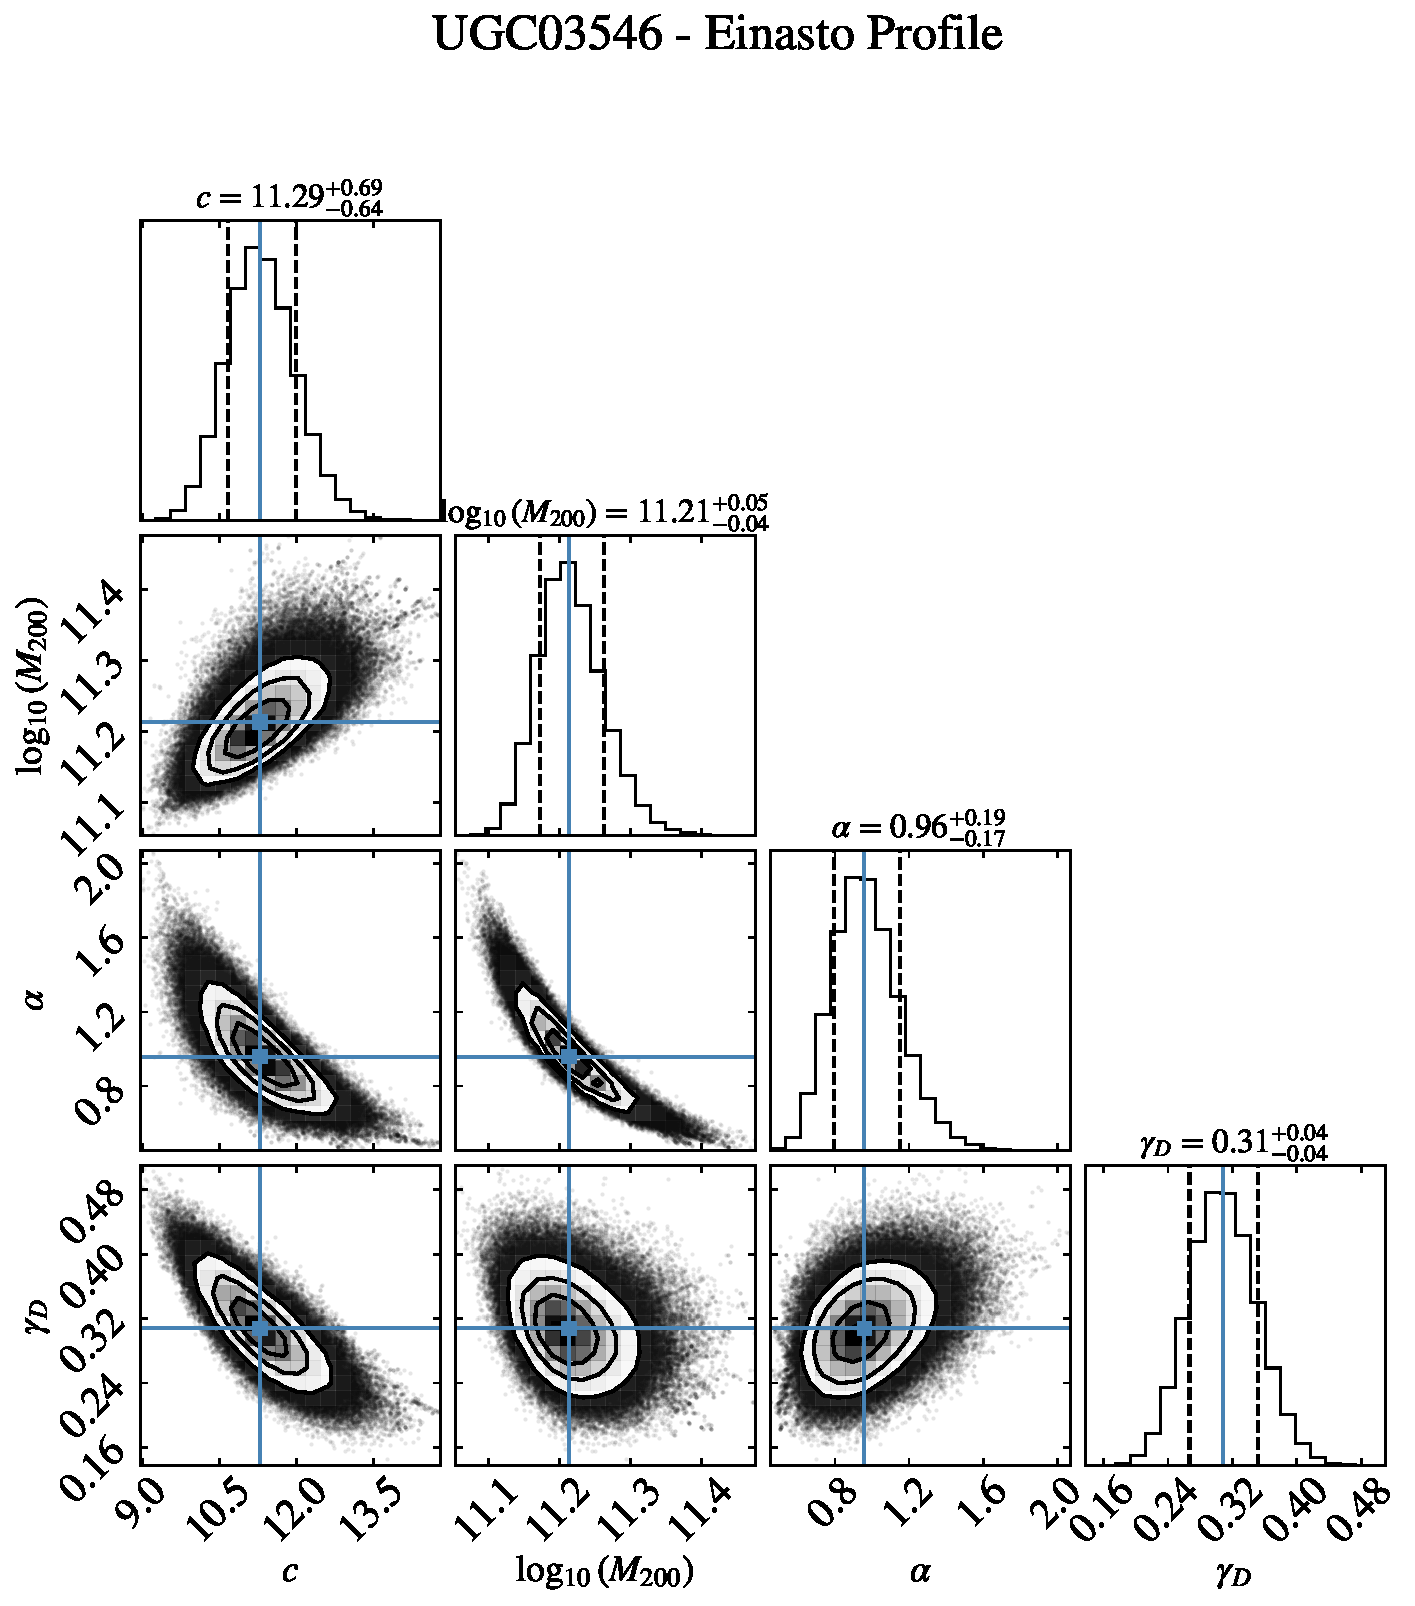
\includegraphics[width=\textwidth]{figs/UGC03546_Eina_Corner.pdf}
        \caption*{UGC03546 (Einasto)}
    \end{minipage}
    \hfill 
    \begin{minipage}[b]{0.48\textwidth}
        \centering
        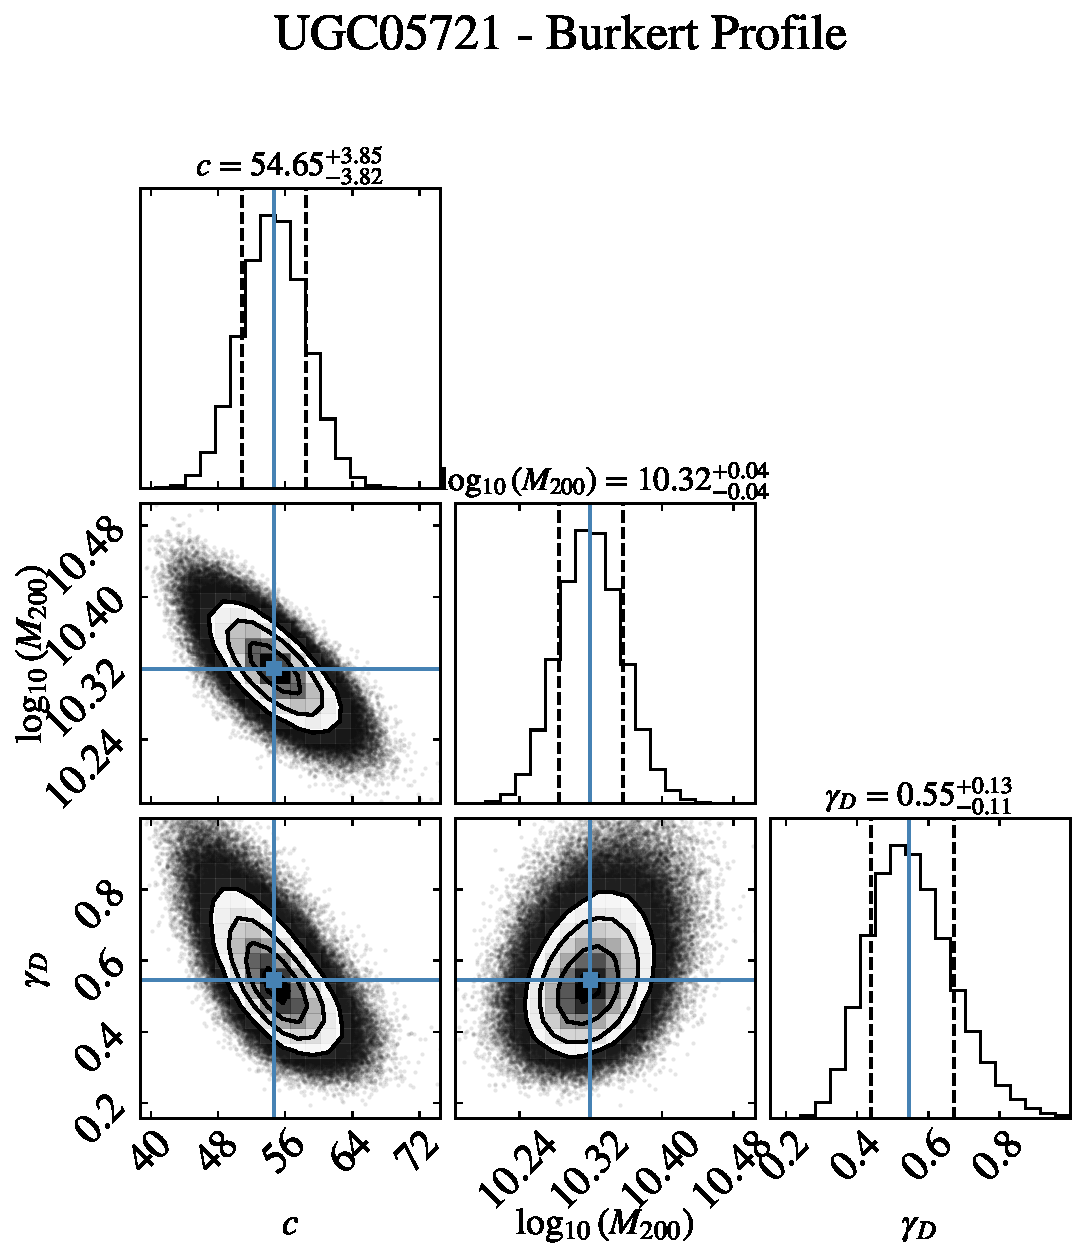
\includegraphics[width=\textwidth]{figs/UGC05721_Burk_Corner.pdf} 
        \caption*{UGC05721 (Burkert)}
    \end{minipage}
    \caption{Exemplos de distribuições de probabilidade posteriores (gráficos de contorno) para os parâmetros amostrados via MCMC. À esquerda, o ajuste do perfil Einasto para a galáxia UGC03546 e, à direita, o ajuste do perfil Burkert para a galáxia UGC05721.}
    \label{fig:corner_plots}
\end{figure}

Um resultado interessante emergiu da análise da relação entre a massa do halo ($M_{200}$) e o parâmetro de concentração ($c$). No contexto do modelo $\Lambda$CDM, espera-se uma anti-correlação, onde halos mais massivos são menos concentrados. Contudo, nossa análise conjunta dos parâmetros de todos os modelos ajustados revelou uma tendência oposta, com uma correlação diretamente proporcional. Essa aparente discrepância pode ser atribuída a um viés introduzido pelo perfil Pseudo-Isotérmico, que, para se ajustar aos dados, frequentemente requer valores de concentração anomalamente altos, distorcendo a relação global.

Em síntese, os resultados obtidos neste trabalho fornecem evidências adicionais contra a universalidade do perfil NFW em escalas galácticas. A metodologia Bayesiana demonstrou ser uma ferramenta poderosa para a análise detalhada de curvas de rotação, e os resultados apontam para uma diversidade na estrutura interna dos halos de matéria escura que desafia as previsões mais simples dos modelos cosmológicos.

%%%%%%%%%%%%%%%%%%%%%%%%%%%%%
\section{Atividades Realizadas e Produtos do Projeto}
Ao longo do período de vigência deste projeto de Iniciação Científica, todas as atividades planejadas foram executadas com sucesso, culminando em uma análise robusta e na produção de resultados científicos relevantes. As tarefas executadas podem ser resumidas da seguinte forma:

Primeiramente, foi realizado um aprofundamento teórico sobre os temas de matéria escura, dinâmica galáctica e métodos estatísticos, consolidando a base de conhecimento necessária para a pesquisa. Em paralelo, foram desenvolvidas as habilidades de programação em \texttt{Python}, com foco nas bibliotecas científicas essenciais para a análise de dados astrofísicos.

A etapa seguinte consistiu na familiarização com o catálogo de dados \texttt{SPARC}. Foi desenvolvido um \textit{pipeline} de software para ler, processar e visualizar as curvas de rotação. Inicialmente, foram implementados ajustes de perfis de matéria escura utilizando métodos de otimização baseados em $\chi^2$ e busca em grade, cujos resultados para diversas galáxias foram apresentados na XLVII Reunião Anual da Sociedade Astronômica Brasileira.

Posteriormente, a metodologia foi refinada para uma abordagem de inferência Bayesiana completa, utilizando MCMC. Essa análise mais sofisticada, aplicada a uma amostra de galáxias HSB e LSB, resultou em um trabalho que foi aceito para apresentação em formato de pôster na conferência internacional \textit{Galaxy Memoirs 2025}, realizada em Armação Buzius, Rio de Janeiro. A análise foi executada utilizando os recursos computacionais do cluster \textit{Sci-Com} do Núcleo Capixaba de Computação Científica (NC3), que foi fundamental para a viabilidade do processamento intensivo exigido pelo MCMC.

\begin{table}[H]
\caption{Lista de atividades previstas e realizadas do Subprojeto.}
\begin{tabularx}{\textwidth}{|X|}
\hline
1 -  Programação em Python \& \textit{Wolfram Language}: constante desenvolvimento. \\
\hline
2 - Potencial gravitacional em gravitação Newtoniana para modelagem de galáxias. \\
\hline
3 - Modelos de matéria escura e gravitação.  \\
\hline
4 - Familiarização com o \textit{sample} de dados SPARC.  \\
\hline
5 - Otimização de $\chi^2$. \\
\hline
6 - Determinação de parâmetros de modelos, com regiões de confiança, a partir de análise Bayesiana. \\
\hline
7 - Atividades complementares: Limpeza dos códigos e preparação para publicação no Github; Apresentação em eventos. \\
\hline
8 - Relatório parcial. \\
\hline
9 - Relatório final. \\
\hline
\end{tabularx}
{\small Fonte: Produção do próprio autor.}
\end{table}

\begin{table}[H]
\caption{Cronograma de atividades do Subprojeto, indicando a conclusão das tarefas.}
\begin{tabularx}{\textwidth}{|l|c|c|c|c|c|c|c|c|c|c|c|c|}
\hline
\rowcolor[gray]{.9}
Atividade &  set & out & nov & dez & jan & fev & mar & abr & mai & jun & jul & ago\\
\hline
1 & \faSmileO  & \faSmileO  & \faSmileO  & \faSmileO   & \faSmileO & \faSmileO  & \faSmileO  & \faSmileO  & \faSmileO  & \faSmileO  & \faSmileO  & \faSmileO \\
\hline
2 & \faSmileO & \faSmileO  & \faSmileO  &   &   &   &   &   &   &   &   &  \\
\hline
3 &   & \faSmileO  & \faSmileO  & \faSmileO  & \faSmileO &   &   &   &   &   &   &  \\
\hline
4 &   & \faSmileO  & \faSmileO  & \faSmileO  &   &  &   &  &  &  &   &  \\
\hline
5 &   &   &  \faSmileO &  \faSmileO  & \faSmileO & \faSmileO  & \faSmileO  &   &   &   &   &  \\
\hline
6 &   &   &   &    &   &   & \faSmileO  &  \faSmileO & \faSmileO  & \faSmileO  & \faSmileO  &  \\
\hline
7 &   &   &   &   &   &   &   &  \faSmileO  & \faSmileO  & \faSmileO  & \faSmileO  & \faSmileO \\
\hline
8 &   &   &   &   &   & \faSmileO  &   &   &   &   &   &   \\
\hline
9 &   &   &   &   &   &   &   &   &   &   &   & \faSmileO  \\
\hline
\end{tabularx}
{\small Fonte: Produção do próprio autor.}
\end{table}

%%%%%%%%%%%%%%%%%%%%%%%%%%%%%
\section{Agradecimentos}
Agradeço ao Programa Institucional de Iniciação Científica (PIIC) da Universidade Federal do Espírito Santo (UFES) e ao Conselho Nacional de Desenvolvimento Científico e Tecnológico (CNPq) pela bolsa e pelo fomento a esta pesquisa. Agradeço também ao Núcleo Capixaba de Computação Científica (NC3) por disponibilizar a infraestrutura computacional do cluster \textit{Sci-Com}, cujos recursos foram indispensáveis para a execução das amostragens MCMC.

%%%%%%%%%%%%%%%%%%%%%%%%%%%%%
\section{Atividades Complementares}
Durante a execução deste projeto, os resultados parciais e finais foram divulgados em importantes fóruns científicos. As principais atividades complementares foram:
\begin{itemize}
    \item \textbf{Apresentação de Pôster:} Participação na XLVII Reunião Anual da Sociedade Astronômica Brasileira (SAB), onde foram apresentados os resultados preliminares da análise de galáxias do catálogo SPARC.
    \item \textbf{Apresentação em Conferência Internacional:} Apresentação de um pôster na conferência \textit{Galaxy Memoirs 2025}, detalhando a análise Bayesiana comparativa entre os perfis de matéria escura em galáxias HSB e LSB.
    \item \textbf{Disponibilização de Código:} O código-fonte em \texttt{Python} desenvolvido para a análise das curvas de rotação está sendo preparado e documentado para publicação em um repositório público no \textit{GitHub}, em alinhamento com as práticas de ciência aberta.
\end{itemize}

%%%%%%%%%%%%%%%%%%%%%%%%%%%%%
\section*{Referências Bibliográficas}
\flushleft{BINNEY, James; TREMAINE, Scott. \textbf{Galactic dynamics}. Princeton university press, 2011.}

\flushleft{BOSMA, A. The distribution and kinematics of neutral hydrogen in spiral galaxies of various morphological types. 1978. \textbf{Thesis (PhD)}. University of Groningen, 1978.}

\flushleft{BURKERT, Andreas. The structure of dark matter halos in dwarf galaxies. \textbf{The Astrophysical Journal}, v. 447, n. 1, p. L25, 1995.}

\flushleft{DE BLOK, W. J. G. The Core‐Cusp Problem. \textbf{Advances in Astronomy}, v. 2010, n. 1, p. 789293, 2010.}

\flushleft{DEL POPOLO, A. \textit{et al}. A unified solution to the small scale problems of the $\Lambda$CDM model. \textbf{Journal of Cosmology and Astroparticle Physics}, v. 2014, n. 04, p. 021, 2014.}

\flushleft{HERNÁNDEZ-ARBOLEDA, Alejandro; RODRIGUES, Davi C. Rotação de galáxias e matéria escura. \textbf{Cadernos de Astronomia}, v. 2, n. 1, p. 6-33, 2021.}

\flushleft{KEETON, Charles. \textbf{Principles of astrophysics}. New York: Springer, 2014.}

\flushleft{LI, Pengfei \textit{et al}. Fitting the radial acceleration relation to individual SPARC galaxies. \textbf{Astronomy \& Astrophysics}, v. 615, p. A3, 2018.}

\flushleft{LELLI, Federico; MCGAUGH, Stacy S.; SCHOMBERT, James M. SPARC: Mass models for 175 disk galaxies with Spitzer photometry and accurate rotation curves. \textbf{The Astronomical Journal}, v. 152, n. 6, p. 157, 2016.}

\flushleft{NAVARRO, Julio F.; FRENK, Carlos S.; WHITE, Simon DM. A universal density profile from hierarchical clustering. \textbf{The Astrophysical Journal}, v. 490, n. 2, p. 493, 1997.}

\flushleft{RODRIGUES, Davi C. \textit{et al}. Evidence against cuspy dark matter haloes in large galaxies. \textbf{Monthly Notices of the Royal Astronomical Society}, v. 470, n. 2, p. 2410-2426, 2017.}

\flushleft{RUBIN, V. C.; FORD, W. K.; THONNARD, N. Extended rotation curves of high-luminosity spiral galaxies. IV - Systematic dynamic properties, SA to SC. \textbf{The Astrophysical Journal}, v. 225, p. L107-L111, 1978.7.}

\flushleft{WALTER, Fabian \textit{et al}. THINGS: The H i nearby galaxy survey. \textbf{The Astronomical Journal}, v. 136, n. 6, p. 2563, 2008.}

\flushleft{ZWICKY, F. The redshift of extragalactic nebulae. \textbf{Helvetica Physica Acta}, v. 6, p. 110-127, 1933.}

\flushleft{ZWICKY, F. On the masses of nebulae and of clusters of nebulae. \textbf{The Astrophysical Journal}, v. 86, p. 217, 1937.}

\end{document}